\documentclass[tikz,border=2pt]{standalone}
\usepackage{fontspec}
\IfFontExistsTF{Times New Roman}{\setmainfont{Times New Roman}}{\setmainfont{Tinos}}
\usepackage{unicode-math}
\setmathfont{STIXTwoMath-Regular.otf}
\usetikzlibrary{arrows.meta}

\definecolor{ink}{HTML}{253139}
\definecolor{blueink}{HTML}{52758A}
\definecolor{linegray}{HTML}{65747E}
\definecolor{framegray}{HTML}{C9D2D8}
\definecolor{safefill}{HTML}{D5E6F1}
\definecolor{overlapfill}{HTML}{F7E6AF}
\definecolor{failurefill}{HTML}{EFC6C1}
\tikzset{
  font=\fontsize{10}{12}\selectfont,
  text=ink,
  small/.style={font=\fontsize{9}{11}\selectfont},
  head/.style={font=\fontsize{10.5}{12}\selectfont\bfseries,text=blueink},
  axis/.style={-{Stealth[length=4.4pt,width=4.6pt]},line width=.7pt,draw=ink}
}
\newcommand{\legendbox}[1]{%
  \tikz[baseline=2.6pt]{\draw[draw=linegray,line width=.55pt,fill=#1]
    (0,0) rectangle (9pt,9pt);}}

\begin{document}
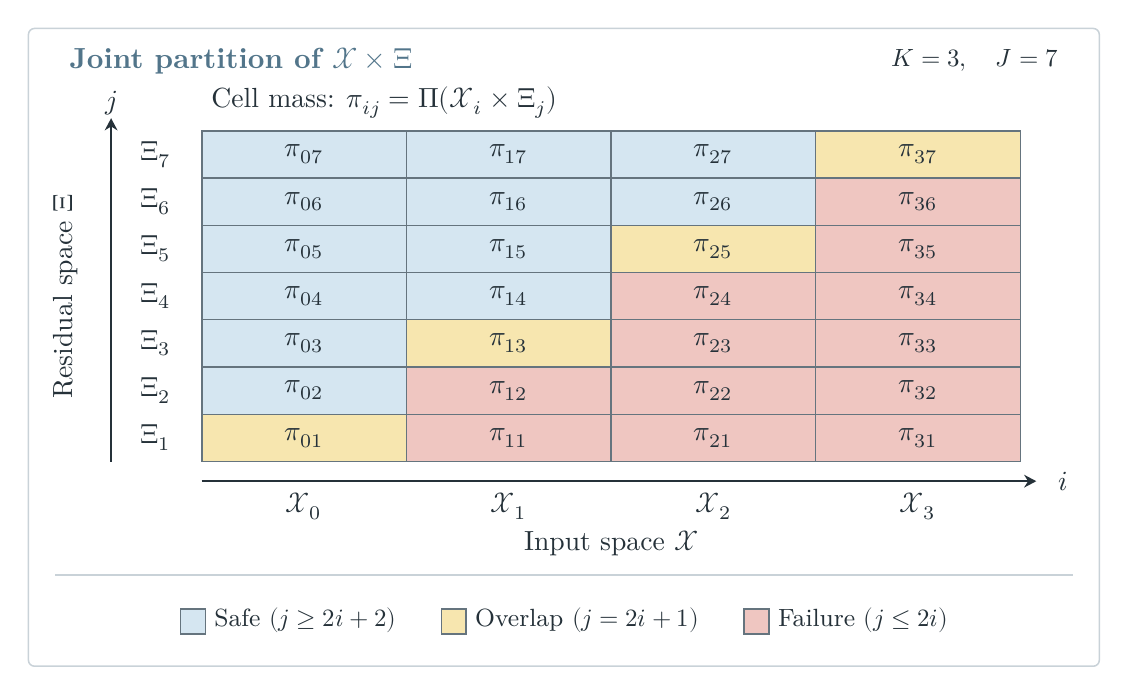
\begin{tikzpicture}[x=1cm,y=1cm]
\draw[draw=framegray,line width=.55pt,rounded corners=2.2pt]
  (0,0) rectangle (13.6,8.1);
\node[head,anchor=west] at (.40,7.69)
  {Joint partition of $\mathcal X\times\Xi$};
\node[small,anchor=east] at (13.20,7.69) {$K=3,\quad J=7$};
\node[anchor=west] at (2.20,7.16)
  {Cell mass: $\pi_{ij}=\Pi(\mathcal X_i\times\Xi_j)$};

% Columns are input cells i=0,...,3. Rows increase upward from j=1 to 7.
% Classification follows manuscript.tex exactly:
% j<=2i: failure; j=2i+1: overlap; j>=2i+2: safe.
\foreach \i in {0,...,3} {
  \foreach \j in {1,...,7} {
    \pgfmathsetmacro{\xl}{2.20+2.60*\i}
    \pgfmathsetmacro{\xr}{\xl+2.60}
    \pgfmathsetmacro{\yb}{2.60+.60*(\j-1)}
    \pgfmathsetmacro{\yt}{\yb+.60}
    \pgfmathsetmacro{\xc}{\xl+1.30}
    \pgfmathsetmacro{\yc}{\yb+.30}
    \pgfmathtruncatemacro{\failurecut}{2*\i}
    \pgfmathtruncatemacro{\overlapcut}{2*\i+1}
    \ifnum\j>\overlapcut
      \def\cellcolor{safefill}
    \else
      \ifnum\j>\failurecut
        \def\cellcolor{overlapfill}
      \else
        \def\cellcolor{failurefill}
      \fi
    \fi
    \fill[\cellcolor] (\xl,\yb) rectangle (\xr,\yt);
    \node at (\xc,\yc) {$\pi_{\i\j}$};
  }
}
% Draw grid lines once to keep their weights uniform.
\foreach \i in {1,...,3} {
  \pgfmathsetmacro{\x}{2.20+2.60*\i}
  \draw[draw=linegray,line width=.45pt] (\x,2.60)--(\x,6.80);
}
\foreach \j in {1,...,6} {
  \pgfmathsetmacro{\y}{2.60+.60*\j}
  \draw[draw=linegray,line width=.45pt] (2.20,\y)--(12.60,\y);
}
\draw[draw=linegray,line width=.65pt] (2.20,2.60) rectangle (12.60,6.80);

% Axis labels and cell names retain the original orientation and notation.
\draw[axis] (1.05,2.60)--(1.05,6.96);
\node at (1.05,7.15) {$j$};
\node[rotate=90] at (.47,4.70) {Residual space $\Xi$};
\foreach \j in {1,...,7} {
  \pgfmathsetmacro{\y}{2.60+.60*(\j-.50)}
  \node[anchor=east] at (1.94,\y) {$\Xi_{\j}$};
}
\draw[axis] (2.20,2.35)--(12.80,2.35);
\node[anchor=west] at (12.96,2.35) {$i$};
\foreach \i in {0,...,3} {
  \pgfmathsetmacro{\x}{2.20+2.60*(\i+.50)}
  \node at (\x,2.03) {$\mathcal X_{\i}$};
}
\node at (7.40,1.56) {Input space $\mathcal X$};

% Center the complete three-item legend, including its swatches and formulas.
\draw[draw=framegray,line width=.45pt] (.34,1.16)--(13.26,1.16);
\node[small,anchor=center,inner sep=0pt] at (6.80,.57) {%
  \legendbox{safefill}\hspace{3pt}Safe $(j\ge2i+2)$\hspace{16pt}%
  \legendbox{overlapfill}\hspace{3pt}Overlap $(j=2i+1)$\hspace{16pt}%
  \legendbox{failurefill}\hspace{3pt}Failure $(j\le2i)$};
\end{tikzpicture}
\end{document}
